\documentclass{article}
    \usepackage[fontset = windowsnew]{ctex}
        \CTEXoptions[today=old]
        \ctexset{figurename=Figure}
    \usepackage{geometry}
        \geometry{left=2.54cm,right=2.54cm,top=2.54cm,bottom=2.54cm}
    \usepackage{amsmath}
    \usepackage{amsfonts}
    \usepackage{siunitx}
    \usepackage{booktabs}
    \usepackage{longtable}
    \usepackage{graphicx}
    \usepackage{subfig}
    \usepackage{float}
    \usepackage{fancyvrb}
    \renewcommand{\labelenumi}{\alph{enumi}.} % Make numbering in the enumerate environment by letter rather than number

    \title{\textbf{数字逻辑与处理器基础实验} \\ [2ex] \begin{large} \emph{32位MIPS处理器设计实验报告} \end{large} }
    \author{王晗 \\ (2013011076)}
    \date{\today}

\begin{document}
    \maketitle

    \begin{table}[htb]
        \centering
        \begin{tabular}{lr}
            Date Performed: & July 15, 2015 \\
            Partners:   & 耿天毅(2012011119) \\
                        & 陈志杰 \fbox{\begin{small}\emph{~~withdrawn~~}\end{small}} \\
        \end{tabular}
    \end{table}

    \section{实验目的}
        熟悉现代处理器的基本工作原理;掌握单周期和流水线处理器的设计方法。

    \section{设计方案}
        \subsection{总体结构}
            由于这次实验涉及的功能较多,我们将完整的CPU分成多个模块。指令存储器、寄存器堆、控制器、ALU控制器、ALU、数据存储器、UART等功能单元均在单独的Module中实现。其中指令存储器、寄存器堆、控制器、ALU控制器、ALU等单元在Single Cycle Core中实例化,作为单周期处理器的核心;数据存储器、UART和定时器、LED、七段数码管、开关在Peripheral中实现,作为处理器的外设。处理器核心和外设在顶层模块中实例化,互相通信。
            
            单周期CPU模块的结构关系如下图所示:
            \begin{figure}[H]
                    \centering
                    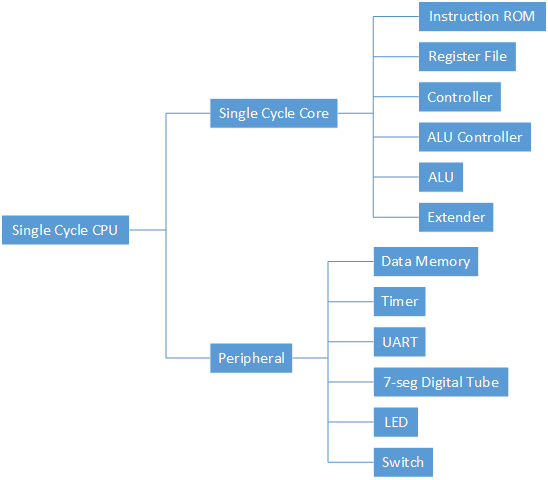
\includegraphics[width=0.62\textwidth]{images/singlecycle.png}
                    \caption{\label{fig:singlecycle}单周期处理器结构}
                \end{figure}
            
            对于流水线CPU,我们还在Pipeline Core中加入了流水线寄存器、冒险检测单元、数据转发单元:
            \begin{figure}[H]
                    \centering
                    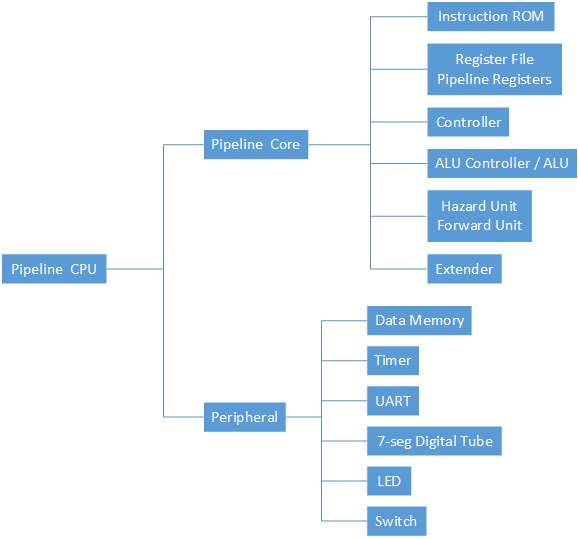
\includegraphics[width=0.62\textwidth]{images/pipeline.png}
                    \caption{\label{fig:pipeline}流水线处理器结构}
                \end{figure}
            
        \subsection{ALU}

        \subsection{寄存器堆和指令存储器}

        \subsection{数据存储器和外设}

        \subsection{控制器和ALU控制器}

        \subsection{单周期数据通路}

        \subsection{流水线数据通路}

        \subsection{汇编代码}
        
        \subsection{汇编器}

    \section{关键代码及文件清单}

    \section{仿真结果及分析}

    \section{硬件调试情况}
        硬件调试情况

    \section{心得体会}

        \begin{enumerate}
            \begin{item}
                我没有
            \end{item}
            \begin{item}
                心得
            \end{item}
            \begin{item}
                体会
            \end{item}
        \end{enumerate}

\end{document}
